\documentclass{article} 
\usepackage{amsmath,amssymb,enumitem,float,fdsymbol,tikz,etoolbox,ifthen,xcolor,fullpage,ulem,graphicx, comment} 




\setlength\parindent{0in}
%\pagestyle{empty}

\everymath{\displaystyle}
\newcommand{\dee}{\,\text{d}}
\newcommand{\diff}[2]{\frac{\text{d}#1}{\text{d}#2}}




\usepackage{physics}
\usepackage{tikz,pgfplots}
\usepackage[siunitx]{circuitikz} %[symbols]
\usepackage[outline]{contour} % glow around text
\usetikzlibrary{arrows,arrows.meta}
\usetikzlibrary{decorations.markings}
\tikzset{>=latex} % for LaTeX arrow head
\usepackage{xcolor}
\colorlet{Icol}{blue!50!black}
\colorlet{Ccol}{orange!90!black}
\colorlet{Rcol}{green!50!black}
\colorlet{loopcol}{red!90!black!25}
\colorlet{pluscol}{red!60!black}
\colorlet{minuscol}{blue!60!black}
\newcommand\EMF{\mathcal{E}} %\varepsilon}
\contourlength{1.5pt}
\tikzstyle{EMF}=[battery1,l=$\EMF$,invert]
\tikzstyle{internal R}=[R,color=Rcol,Rcol,l=$r$,/tikz/circuitikz/bipoles/length=30pt]
\tikzstyle{loop}=[->,red!90!black!25]
\tikzstyle{loop label}=[loopcol,fill=white,scale=0.8,inner sep=1]
\tikzstyle{thick R}=[R,color=Rcol,thick,Rcol,l=$R$]
\tikzstyle{thick C}=[C,thick,color=Ccol,Ccol,l=$C$]
\tikzstyle{myswitch}=[closing switch,line width=0.3] %-{Latex[length=3]},

\setlength\parindent{0in}
\pagestyle{empty}

\begin{document}

\large{\textbf{ASSIGNMENT 2}}

\normalsize

\

\begin{tabular*}{6.5in}{c}
\hline
\end{tabular*}


% Students: edit in your names here or these people will get credit for your work 

\begin{itemize}
    \item \#12345678 Sirius {\bf Black} 
    \item \#24681012 Luna {\bf Lovegood}
    \item \#87654321 Neville {\bf Longbottom}
    \item \#12108642 Albus {\bf Dumbledore}
    \textcolor{red}{\item \#00000000 Mundungus {\bf Fletcher}  (non-contributing)}
\end{itemize}

\begin{tabular*}{6.5in}{c}
\hline
\end{tabular*}

\ 

\textit{Reflection questions encourage you to think about how mathematics is done. This is an important ingredient of success. Reflection questions contribute to your \textbf{engagement grade}.}

\begin{enumerate}[leftmargin=*] 

\item Consider the differences between the types of questions on the previous written assignment, Assignment 1, and the types of questions on your high school math assignments. In one or two paragraphs, describe one major difference, and explain how you might approach assignments in this course differently. Be specific and provide details.

\color{blue}
\textbf{Answers} \newline 
Student answer goes here.
\color{black}


%(All assignments include a \textit{reflection question} designed to encourage you to think deeply about how mathematics is done.)
\end{enumerate}

\begin{tabular*}{6.5in}{c}
\hline
\end{tabular*}

\


A \textit{capacitor} is a basic circuit element that can store charge. 

\

A simple form of capacitor is a pair of conducting plates separated by a dielectric (non-conducting) material. There are other geometries possible such are rolling thin conducting plates and a malleable separating dielectric material into a cylindrical shape, all the while preserving the separation of the two plates. 

\

By attaching a battery, say, to the capacitor, we can store charge from the battery in the capacitor for use at a later time. The capacitor can then become a source of current in the circuit, at least until the capacitor has discharged.

\
\begin{enumerate}
 \setcounter{enumi}{1}


\item ($\bigstar\bigstar\bigstar\largewhitestar$) Suppose we have a capacitor of capacitance $C$ in a circuit with both a resistor of resistance $R$ and a battery with emf $\cal{E}$. All three of these values are constant. This circuit is shown in Figure 1. Note there is a current $I$, which is equal to the rate at which the charge $Q$ changes in time $t$; that is, $I=dQ/dt$. We wish to study $Q(t)$, the charge on the capacitor as a function of time.

\begin{figure}[h]
\begin{center}
% RC+EMF with CLOSED switch
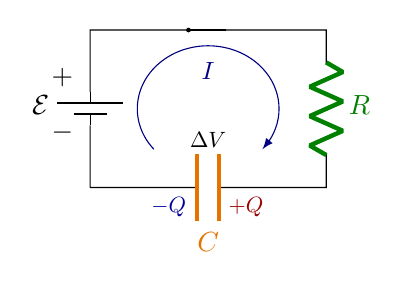
\begin{tikzpicture}
  \def\ang{220}
  \def\a{0.9}
  \def\b{0.8}
  \draw[->,Icol] ({1.5+\a*cos(\ang)},{1+\b*sin(\ang)}) arc (\ang:-40:{\a} and {\b})
                 node[midway,below=3,scale=0.9] {$I$};
  \draw (0,0) to[EMF] (0,2) --++(3,0)
              to[thick R] ++(0,-2) to[thick C] (0,0);
  \fill[black] (1.25,2) circle (0.03);
  \draw[line width=0.6] (1.25,2) --++ (0.48,0);
  \node at (-0.35,0.7) {$-$};
  \node at (-0.35,1.4) {$+$};
  \node[minuscol,scale=0.8] at (1.0,-0.25) {$-Q$};
  \node[pluscol,scale=0.8] at (1.98,-0.25) {$+Q$};
  \node[scale=0.8] at (1.5,0.6) {$\Delta V$};
\end{tikzpicture}
\caption{An $RC$-circuit with an EMF (battery)}
\end{center}
\end{figure}

We can apply Ohm's Law to this circuit to find that 
\[
 {\cal E} -IR -\frac{Q}{C} = {\cal E} - \frac{dQ}{dt} R - \frac{Q}{C} = 0.
\]
Note that this is a differential equation for the function $Q(t)$, which we rearrange as
\begin{equation}
\frac{dQ}{dt} = \frac{{\cal E}}{R} - \frac{Q}{RC}.
\end{equation}

\begin{enumerate}

\item Let us assume the capacitor has no charge on it at time $t=0$. That is, $Q(0)=0$. Confirm that \[
Q(t) = C{{\cal E}\left(1-e^{-t/RC}\right)}
\]
is a solution of the differential equation (3) with the initial condition $Q(0)=0$.

\item Sketch a graph of $Q(t)$.

\item What is $\lim_{t\to \infty} Q(t)$? What can you conclude about the charge on the capacitor from this result?

\item Find an expression for the current $I(t)$. 

\item What can you conclude about the behaviour of this circuit after a long time passes?
\end{enumerate}



\color{blue}
\textbf{Answers}
\begin{enumerate}
    \item Student answer goes here.
    \item Student answer goes here.
    \item Student answer goes here.
    \item Student answer goes here.
    \item Student answer goes here.
\end{enumerate}
\color{black}

\item ($\bigstar\bigstar\bigstar\largewhitestar$) Suppose now we remove the battery from the circuit, as shown in Figure 2.  

\begin{figure}[h]
\begin{center}
% RC with CLOSED switch
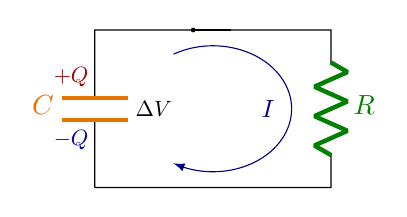
\begin{tikzpicture}
  \def\ang{120}
  \def\a{1.0}
  \def\b{0.8}
  \draw (0,0) to[thick C] (0,2) --++(3,0)
              to[thick R] ++(0,-2) -- (0,0);
  \fill[black] (1.25,2) circle (0.03);
  \draw[line width=0.6] (1.25,2) --++ (0.48,0);
  \node[minuscol,scale=0.8] at (-0.3,0.6) {$-Q$};
  \node[pluscol,scale=0.8] at (-0.3,1.4) {$+Q$};
  \node[scale=0.8] at (0.75,1) {$\Delta V$};
  \draw[->,Icol] ({1.5+\a*cos(\ang)},{1+\b*sin(\ang)}) arc (\ang:-120:{\a} and {\b})
                 node[midway,left=3,scale=0.9] {$I$};
\end{tikzpicture}
\caption{An $RC$ circuit with no EMF (battery)}
\end{center}
\end{figure}

\begin{enumerate}

\item Write down the differential equation that comes form Ohm's Law for the circuit shown in Figure 2.

\item Suppose that the capacitor is the value of $Q$ you found in Question 1(c); call this value $Q_{\max}$. Write down the solution $Q(t)$ to the differential equation you found in part (a) satisfying the initial condition $Q(0) = Q_{\max}$.

\item Sketch a graph of $Q(t)$.

\item Find an expression for the current $I(t)$.  

\item What can you conclude about the behaviour of this circuit after a long time passes?

\end{enumerate}



\color{blue}
\textbf{Answers}
\begin{enumerate}
    \item Student answer goes here.
    \item Student answer goes here.
    \item Student answer goes here.
    \item Student answer goes here.
    \item Student answer goes here.
\end{enumerate}
\color{black}

\item ($\bigstar\bigstar\bigstar\largewhitestar$) The quantity $\tau = RC$ that appears in the solutions for $Q(t)$ in these $RC$-circuits is a time constant characteristic of these circuits; it has dimensions (units) of time and is a useful quantity to consider in practical applications.

\begin{enumerate}
    \item Calculate $Q(\tau)$ for the $RC$ circuit without the battery assuming the initial charge on the capacitor is $Q_0 \neq 0$.  Now, calculate $Q(\tau)$ for the circuit with the battery assuming the initial charge on the capacitor is 0.  What does $\tau$ measure in each of these cases?

    \item Engineers generally consider a charging capacitor starting with zero charge to be fully charged after a time period of $5\tau$.  They also consider a fully charged but discharging capacitor to be fully discharged after a time period of $5\tau$. Use calculations to help you explain why this practice can be considered reasonable?

    \item Assume the initial charge on a capacitor is zero and it is put in series with a resistor and an emf. Sketch the graph of the piecewise function giving the charge $Q(t)$ on this capacitor that results if you first charge the capacitor for a time period of $5\tau$ in this circuit, and then remove the emf from the circuit, leaving only the resistor and capacitor in series, and measure the charge on the capacitor for a period $5\tau$ afterwards. Assume you can remove the emf instantaneously from the circuit. 

  

\end{enumerate}

\color{blue}
\textbf{Answers}
\begin{enumerate}
    \item Student answer goes here.
    \item Student answer goes here.
    \item Student answer goes here.
\end{enumerate}
\color{black}

\end{enumerate}





\hrulefill



\end{document}
